\section{紧算子的非零谱}
\label{sec:ospec-compact-spectrum}

乘法算子和右移算子的谱里都有大块的区域，因为它们在无穷多个方向上都保持可观的大小：乘法算子的对角元$x$不趋于零，右移保持长度。紧算子则相反，它把有界集压成几乎有限的集合，越来越多的方向被压得越来越小。对角情形最清楚：$a_n\to0$时，$\operatorname{diag}(a_n)$可以被有限截断按算子范数逼近，所以是紧算子；$a_n$不趋于零时，有一列下标使$\lvert a_{n_k}\rvert\geq\delta>0$，单位向量$e_{n_k}$的像彼此至少相距$\sqrt2\,\delta$，算子不紧。

本节证明，这种压缩使非零谱点回到矩阵的情形：它们都是特征值，特征空间有限维，并且特征值只能向零聚集。连续谱被赶到了$0$这一个点上。

本节设$X$是复Banach空间，$T\in\mathcal B(X)$是紧算子。证明反复用到两个事实。第一，紧算子与有界算子的复合仍紧：若$K$紧、$A$有界，有界输入列经$K$后有收敛子列，再经连续的$A$仍收敛，所以$AK$紧；$KA$把有界列先变成有界列，再由$K$抽出收敛子列，所以$KA$也紧。

第二是第~\ref{chap:functions-as-vectors}章用来证明无限维闭球不紧的Riesz引理。在Hilbert空间中，单位向量可以取在子空间的正交补里，与子空间距离恰为$1$；Banach空间没有正交性，Riesz引理提供一个距离至少为$\theta$的替代品。

\begin{lemma}[Riesz引理]
\label{lem:ospec-riesz}
设$X$是赋范空间，$M\subsetneq X$是闭子空间，$0<\theta<1$。则存在单位向量$x\in X$，使$\lVert x-m\rVert\geq\theta$对一切$m\in M$成立。
\end{lemma}

\begin{proof}
取$x_0\notin M$。$M$闭，所以$d=\operatorname{dist}(x_0,M)>0$。由下确界的定义，存在$m_0\in M$使$\lVert x_0-m_0\rVert\leq d/\theta$。令$r=\lVert x_0-m_0\rVert$，$x=(x_0-m_0)/r$。对任意$m\in M$，点$m_0+rm$仍属于$M$，所以
\[
\lVert x-m\rVert=\frac{\lVert x_0-(m_0+rm)\rVert}{r}\geq\frac{d}{d/\theta}=\theta .
\]
\end{proof}

\paragraph{紧算子减去非零数乘}
矩阵中“单射推出可逆”的一个关键部分，是单射时存在正的放大下界。下面的引理说明，紧算子减去非零数乘时这一点仍然成立。

\begin{lemma}[单射推出下有界]
\label{lem:ospec-bounded-below}
设$K\in\mathcal B(X)$紧，$\mu\neq0$，且$K-\mu I$是单射。则存在$c>0$使
\begin{equation}
\lVert(K-\mu I)x\rVert\geq c\lVert x\rVert\qquad(x\in X),
\label{eq:ospec-bounded-below}
\end{equation}
从而$\operatorname{Ran}(K-\mu I)$是闭子空间。
\end{lemma}

\begin{proof}
反设不存在这样的$c$，可取单位向量$x_n$使$(K-\mu I)x_n\to0$。由紧性，可抽子列使$Kx_n\to y$。于是
\[
\mu x_n=Kx_n-(K-\mu I)x_n\to y,
\]
即$x_n\to x=y/\mu$，且$\lVert x\rVert=1$。由连续性$(K-\mu I)x=0$，这与单射矛盾。像闭的论证与引理~\ref{lem:ospec-approx-eigen}相同：下界使原像列成为柯西列，由$X$的完备性取极限即可。
\end{proof}

这里$\mu\neq0$是必需的。$\mu=0$时结论不成立，例如第~\ref{chap:linear-operators}章的对角算子$A(x_n)=(x_n/n)$是单射，而$\lVert Ae_n\rVert=1/n$，没有正的下界。

\begin{theorem}[紧算子的非零谱]
\label{thm:ospec-compact-spectrum}
设$X$是复Banach空间，$T\in\mathcal B(X)$紧，$\lambda\neq0$。则：
\begin{enumerate}
\item 特征空间$\ker(T-\lambda I)$有限维；
\item 若$T-\lambda I$是单射，则它是满射，从而$\lambda\in\rho(T)$；因此每个非零谱点都是特征值；
\item 对每个$\delta>0$，满足$\lvert\lambda\rvert\geq\delta$的特征值只有有限个；因此$\sigma(T)\setminus\{0\}$至多可数，并且只能在$0$处聚集；
\item 若$X$无限维，则$0\in\sigma(T)$。
\end{enumerate}
\end{theorem}

证明的共同思路是：若某个结构无限大，就能用Riesz引理造出一列彼此远离的单位向量，它们的像仍彼此远离，这与紧性矛盾。

\begin{proof}
（1）记$N=\ker(T-\lambda I)$，它是闭子空间，$T$在$N$上等于$\lambda I$。若$N$无限维，由Riesz引理可逐个取单位向量$y_1,y_2,\ldots\in N$，使$y_n$与$\operatorname{span}\{y_1,\ldots,y_{n-1}\}$的距离至少为$\frac12$；有限维子空间是闭的，所以引理适用。于是对$n\neq m$，
\[
\lVert Ty_n-Ty_m\rVert=\lvert\lambda\rvert\,\lVert y_n-y_m\rVert\geq\frac{\lvert\lambda\rvert}{2}.
\]
有界列$(y_n)$的像没有收敛子列，与紧性矛盾。

（2）记$B=T-\lambda I$，反设它是单射而不满射。对$n\geq1$，二项式展开给出
\[
B^n=(-\lambda)^nI+TP_n(T),
\]
其中$P_n(T)$是$T$的多项式。所以$B^n=K_n-\mu_nI$，其中$K_n=TP_n(T)$紧，$\mu_n=-(-\lambda)^n\neq0$。$B^n$是单射的复合，仍是单射，由引理~\ref{lem:ospec-bounded-below}，$Y_n=\operatorname{Ran}B^n$是闭子空间，并且
\[
X=Y_0\supseteq Y_1\supseteq Y_2\supseteq\cdots.
\]

这些包含都是严格的。$Y_1\neq Y_0$是假设。若有$n\geq1$使$Y_{n+1}=Y_n$，取最小的这样的$n$，再取$z\in Y_{n-1}\setminus Y_n$。则$Bz\in Y_n=Y_{n+1}$，可写
\[
Bz=B^{n+1}w=B(B^nw).
\]
由$B$单射，$z=B^nw\in Y_n$，矛盾。

由Riesz引理，对每个$n\geq1$取单位向量$y_n\in Y_n$，使其与$Y_{n+1}$的距离至少为$\frac12$。设$n<m$，用$T=B+\lambda I$改写
\[
Ty_n-Ty_m=\lambda y_n-z,\qquad z=-By_n+By_m+\lambda y_m .
\]
其中$By_n\in Y_{n+1}$，$By_m\in Y_{m+1}\subseteq Y_{n+1}$，$y_m\in Y_m\subseteq Y_{n+1}$，所以$z\in Y_{n+1}$，从而
\[
\lVert Ty_n-Ty_m\rVert=\lvert\lambda\rvert\,\Bigl\lVert y_n-\frac{z}{\lambda}\Bigr\rVert\geq\frac{\lvert\lambda\rvert}{2}.
\]
$(Ty_n)$没有收敛子列，与紧性矛盾。所以$B$是满射；它是有界双射，由有界逆定理$\lambda\in\rho(T)$。

（3）反设有无穷多个互不相同的特征值$\lambda_1,\lambda_2,\ldots$，$\lvert\lambda_n\rvert\geq\delta$，相应特征向量为$x_n$。先证它们线性无关。若有非平凡的线性关系，取项数最少的一个$\sum_{i\leq k}a_ix_i=0$，所有$a_i\neq0$且$k\geq2$。作用$T-\lambda_kI$，得
\[
\sum_{i<k}a_i(\lambda_i-\lambda_k)x_i=0,
\]
这是项数更少的非平凡关系，矛盾。

令$M_n=\operatorname{span}\{x_1,\ldots,x_n\}$，它们严格递增且闭，并且$(T-\lambda_nI)M_n\subseteq M_{n-1}$。由Riesz引理取单位向量$y_n\in M_n$，使其与$M_{n-1}$的距离至少为$\frac12$。对$n>m$，
\[
Ty_n-Ty_m=\lambda_ny_n-\bigl((\lambda_nI-T)y_n+Ty_m\bigr),
\]
括号中两项分别属于$M_{n-1}$与$M_m\subseteq M_{n-1}$，所以
\[
\lVert Ty_n-Ty_m\rVert\geq\frac{\lvert\lambda_n\rvert}{2}\geq\frac\delta2.
\]
这与紧性矛盾。结合（2），满足$\lvert\lambda\rvert\geq\delta$的谱点只有有限个，令$\delta=1,\frac12,\frac13,\ldots$即得其余结论。

（4）若$0\in\rho(T)$，则$I=T^{-1}T$是有界算子与紧算子的复合，是紧算子；但无限维空间中恒等算子不紧（第~\ref{chap:linear-operators}章），矛盾。
\end{proof}

结论（2）保留了矩阵的“单射推出可逆”：对$\lambda\neq0$，方程$(T-\lambda I)u=g$的唯一性已经推出对一切$g$的可解性与稳定性。乘法算子的谱$[0,1]$不可数，所以$M$不是紧算子，这与对角元不趋于零相符。

结论（4）说明$0$是例外，它在无限维中总是谱点，却不一定是特征值。下面两个例子都表明这一点，也说明$0$处正是连续谱待着的地方。

\paragraph{对角算子}
在$\ell^2$上令$A(x_n)=(x_n/n)$，第~\ref{chap:linear-operators}章已证明它紧。由$Ae_k=e_k/k$，每个$1/k$都是特征值，特征空间由$e_k$张成，是一维的。

$A$是单射，$0$不是特征值。像包含一切有限支撑序列，所以稠密；由定理的结论（4），$0\in\sigma(A)$，因此$0\in\sigma_{\mathrm c}(A)$。例如$y=(1/n)$不在像中，因为解$x_n=ny_n=1$不平方可和。

记$S_A=\{1/n:n\geq1\}\cup\{0\}$。若$\lambda\notin S_A$，则$d=\operatorname{dist}(\lambda,S_A)>0$，方程$(A-\lambda I)x=y$逐分量解出
\[
x_n=\frac{y_n}{1/n-\lambda},\qquad\lVert x\rVert\leq\frac{\lVert y\rVert}{d}.
\]
所以$\lambda\in\rho(A)$，$\sigma(A)=S_A$。取$y=e_n$并让$1/n$逼近离$\lambda$最近的谱点，可知上面的界不能改进，于是
\begin{equation}
\lVert R_\lambda\rVert=\frac{1}{\operatorname{dist}(\lambda,\sigma(A))}\qquad(\lambda\in\rho(A)).
\label{eq:ospec-diagonal-resolvent}
\end{equation}

图~\ref{fig:ospec-spectrum-resolvent}画出了这些谱点与预解范数。每个$1/n$附近范数都趋于无穷，就像矩阵的特征值；不同的是这些尖峰无穷多，并向$0$聚集。

\begin{BookInlineFigure}
  \centering
  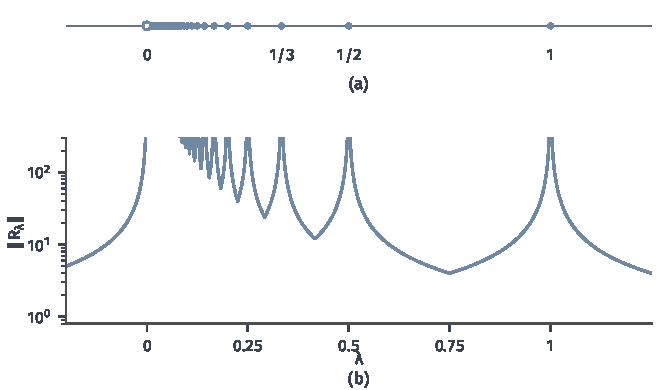
\includegraphics[width=112mm]{figures/04-spaces-measures-and-geometry/03-function-spaces/matplotlib/ospec-spectrum-resolvent/figure.pdf}
  \caption{$\ell^2$上$A(x_n)=(x_n/n)$的谱。(a)~特征值$1/n$（实心点）向$0$聚集，$0$属于谱但不是特征值（空心点）。(b)~实参数$\lambda$处预解算子的范数，纵轴取对数；各谱点处的尖峰向$0$聚集，靠近$0$时尖峰之间的低谷也越出了纵轴范围。}
  \label{fig:ospec-spectrum-resolvent}
\end{BookInlineFigure}

\paragraph{累积积分没有特征值}
紧性保证了非零谱点的有限维结构，却不保证有足够多的特征向量。在$L^2(0,1)$上令
\[
(Vf)(x)=\int_0^xf(t)\,\mathrm dt.
\]
它的核$\mathbf 1_{\{t<x\}}$平方可积，由第~\ref{chap:linear-operators}章，$V$是紧算子。

设$Vf=\lambda f$，$\lambda\neq0$。右端$Vf$连续，所以$f=\lambda^{-1}Vf$连续；于是$Vf$连续可导，$f$也连续可导。对$Vf=\lambda f$求导，并在$x=0$处取值，得到
\[
\lambda f^\prime=f,\qquad f(0)=\lambda^{-1}(Vf)(0)=0.
\]
这个初值问题的解是$f(x)=f(0)\mathrm e^{x/\lambda}=0$，所以$V$没有非零特征值。

$\lambda=0$也不是特征值。$Vf=0$说明$f$在每个区间$[0,x]$上积分为零，相减后在每个区间上积分为零。区间示性函数的线性组合在$L^2(0,1)$中稠密（第~\ref{chap:wavelet-transform}章），$f$与一个稠密集正交，只能为零。

由定理~\ref{thm:ospec-compact-spectrum}，非零谱点都是特征值，因此$\sigma(V)=\{0\}$，而$V$一个特征向量也没有。像的情况也可以判定：$V^*g(t)=\int_t^1g$，同样的论证给出$\ker V^*=\{0\}$，所以$V$的像稠密，$0$属于连续谱。

离散化可以看出这件事的矩阵对应物。把$[0,1]$分成$n$段，取$h=1/n$，累积积分变成$(\bm V_n\bm x)_i=h\sum_{j\leq i}x_j$，它是下三角矩阵，对角元全是$h$。特征值只有$h$，随$n$增大趋于$0$，与$\sigma(V)=\{0\}$相符；而$\bm V_n-h\bm I$的秩是$n-1$，整个矩阵只有一个特征方向。特征方向的严重不足，到了无限维就成了一个也没有。

\paragraph{五个例子的比较}
表~\ref{tab:ospec-gallery}汇总了本章到目前为止的算子。前三个不是紧算子，谱可以是区间或圆盘；后两个紧，谱都收缩到可数集，连续谱只剩$\{0\}$。

\begin{table}[!htb]
  \centering
  \caption{五个算子的谱。$M$是$L^2(0,1)$上乘以$x$的算子，$S$与$L$是$\ell^2$上的右移与左移，$A=\operatorname{diag}(1/n)$，$V$是累积积分；$\mathbb D$表示开单位圆盘，$\mathbb T$表示单位圆周。}
  \label{tab:ospec-gallery}
  \begin{tabular}{@{}cllll@{}}
    \toprule
    算子 & 谱 & 点谱 & 连续谱 & 剩余谱\\
    \midrule
    $M$ & $[0,1]$ & $\varnothing$ & $[0,1]$ & $\varnothing$\\
    $S$ & $\overline{\mathbb D}$ & $\varnothing$ & $\mathbb T$ & $\mathbb D$\\
    $L$ & $\overline{\mathbb D}$ & $\mathbb D$ & $\mathbb T$ & $\varnothing$\\
    $A$ & $\{1/n\}\cup\{0\}$ & $\{1/n\}$ & $\{0\}$ & $\varnothing$\\
    $V$ & $\{0\}$ & $\varnothing$ & $\{0\}$ & $\varnothing$\\
    \bottomrule
  \end{tabular}
\end{table}

表中$L$的圆周部分这样判定：$\lvert\lambda\rvert=1$时，特征方程的解$(c,c\lambda,c\lambda^2,\ldots)$不平方可和，所以$L-\lambda I$是单射；由$\ker(S-\bar\lambda I)=\{0\}$，它的像稠密；谱是闭集，圆周属于谱。

两个紧算子的对比划出了本节结论的边界。紧性把非零谱变成离散的特征值，但不保证特征向量张满空间，更不保证它们彼此正交；$V$的谱只有一个点，任何沿特征方向的展开都不存在。下一节加入自伴条件，正是为了得到正交而完备的特征方向。
